\documentclass[a4paper,11pt]{extarticle} %este tipo de doc ofrece más tamaños de letra

\usepackage[utf8]{inputenc}%codificación
\usepackage{csquotes}
\usepackage[spanish, mexico]{babel}%Paquete de caracteres y títulos en español de méxico

\usepackage{amsmath, mathtools}%Paquete para insertar símbolos matemáticos
\usepackage[bitstream-charter]{mathdesign}
\usepackage{textcomp}
\usepackage{textcomp,gensymb}
\usepackage[table,xcdraw, dvipsnames]{xcolor}
\usepackage{fontenc}

\usepackage[shortlabels]{enumitem}

\usepackage[tmargin= 1.7cm,bmargin=1.7cm,lmargin=1.7cm,rmargin=1.7cm]{geometry}

%estos son para tablas y figuras
\usepackage{float}%Paquete para tratar figuras y tablas como flotantes
\usepackage{graphicx}
\usepackage{svg}
\usepackage{caption}
\usepackage{subcaption}
\usepackage{physics}

\usepackage{verbatim}%comentarios en bloque

\captionsetup{font=footnotesize,labelfont=footnotesize} % hace al caption mas chiquito

%convierte los cuadros del caption en tablas
\renewcommand{\listtablename}{Índice de tablas}
\renewcommand{\tablename}{Tabla}

% si quieren usar alfabeto griego sin entrar en mathmode
\usepackage{textgreek}

\usepackage{adjustbox} % para ajustar tablas

\usepackage{url}%Paquete para insertar URL's
\usepackage{hyperref}

\usepackage{multicol}%Paquete para crear ambientes multicolumna
\setlength\columnsep{16pt}%Especifíca separación de las columnas

%este es para la bibliografía yo uso ieee pero se puede cambiar
\usepackage[
backend=biber,
bibencoding=utf8,
style=ieee,
sorting=none
]{biblatex}
\addbibresource{tarea2entro.bib}


% otros nuevos comandos personalizados.
%\newcommand{\dbar} {\ensuremath{\,\mathchar'26\mkern-12mu d}}

 \newcommand{\cita}[1]{\textsuperscript{\textbf{\cite{#1}}}} % este es para que la cita se vea en superíndice para ieee, si usan otro formato bórrenlo
 \newcommand{\ut}[1]{\textbf{#1}} %les hace escribir menos si quieren poner negritas en texto y mate
 \newcommand{\um}[1]{\mathbf{#1}}
 \renewcommand{\thefootnote}{\Roman{footnote}} %los pie de pagina los pone en letras romanas
 \newcommand{\dbar}{\text{\dj}}
 
\begin{document}

% TITULO ------------------------------------------------------------------------

\begin{center}

    \Large{\textbf{Ejercicios Entropía.}}

    %--------------------------------------------------------------------------------

    % INFO CONTACTO -----------------------------------------------------------------

    \vspace{0.35em}

    \urlstyle{same}
    \small{\textbf{ Pérez Flores Julio Alfonso,}
        \textit{\href{mailto:julio_ perez@ciencias.unam.mx}{julio\textunderscore perez@ciencias.unam.mx}}} \linebreak
    \small{\textbf{ Méndez Martínez Yuvia Libertad,}
        \textit{\href{mailto:yuviali1614@ciencias.unam.mx}{yuviali1614@ciencias.unam.mx}}} \linebreak
    \textit{\small{Facultad de Ciencias, Universidad Nacional Autónoma de México. }}

    \vspace{0.65em}

    \small{ 25 de Marzo, 2023.}

\end{center}


\begin{enumerate}[label=\textbf{\arabic*}), leftmargin=*]

    %==================================================================%
    % Ejercicio 1
    %==================================================================%

    \item Al efectuar una expansión adiabática y reversible de un gas ¿Cuál es la variación de entropía?

    \vspace{\baselineskip}

    \begin{enumerate}
    \item  \includegraphics*[H]{T-S.png}
    \item  Como se trata de un proceso reversible  sabemos que:
    \[ \dbar Q =TdS \]
   El proceso de $A$ a $B$ se trata de un proceso isotermico, por lo que si integramos la expresión anterior tenemos:
   \[ \int \dbar Q =T_{c}\int dS \]
   \[ \Rightarrow \int _v_A ^v_B \dbar Q = T_{c} \Delta S\]
   \[nRT_c \ln \left( \frac{v_B}{v_A}\right) = T_{c}\Delta S = Q_{entrada}\]
    En el proceso de $B$ a $C$ al tratarse de un proceso adiabático, no hay intercambio de calor $\Rightarrow Q=0$\\

    En  el proceso de $C$ a $D$ tenemos un proceso isotermico, por lo que analogamente al proceso de $A$ a $B$ tenemos:

\[ \int \dbar Q =T_{f}\int dS \]
   \[ \Rightarrow \int _v_C ^v_D \dbar Q = T_{f} \Delta S\]
   \[nRT_c \ln \left( \frac{v_D}{v_C}\right) = T_{f}\Delta S = Q_{salida}\]
   Al tratarse de un calor de salida:
   \[ Q_{salida }= -nRT_c \ln \left( \frac{v_D}{v_C}\right) \]

   Ahora bien si  se trata de un gas ideal y el proceso se realiza a presión constante tenemos que:
   \[ \frac{v_1}{T_1}=\frac{v_2}{T_2}\]
   \[\Rightarrow \frac{T_2}{T_1}=\frac{v_2}{v_1}\]

Entonces tenemos que:
\[ \frac{v_B}{v_A}=\frac{Tf}{Tc}=\frac{v_D}{v_c}\]




\end{enumerate}


    \vspace{\baselineskip}

    %==================================================================%
    % Ejercicio 2
    %==================================================================%

    \item{ 1 \ut{kg} de agua se encuentra a 0 \ut{°C} y se calienta hasta 100 \ut{°C}. Calcúlese la variación
                de entropía
          }

    \vspace{\baselineskip}

    
Podemos apreciar que este sistema se encuentra a una presión constante
pues se ebulle a presión atmosférica por lo tanto podemos aprovechar 
la definición de C\textsubscript{p}.

\begin{gather*}
    C_{p}\ =\ \frac{\dbar Q_{p}}{mdT}\ \ \ \Rightarrow\ \ \
    \dbar Q_{p}\ =\ mC_{p}dT\ \ \ \Rightarrow\\
    dS_{p}\ =\ \frac{mC_{p}}{T}\ dT\ \ \ \therefore\\
    \\
    \Delta S\ = mC_{p} \int_{273.15\ \um{K}}^{373.15\ \um{K}}\ \frac{1}{T}\ dT\ =\
    mC_{p} \ln{\left(\frac{373.15\ \um{K}}{273.15\ \um{K}}\right)}\\ 
    \\
    \shortintertext{utilizando el valor de C\textsubscript{p} registrado por Engineering ToolBox\cita{Engineering}}\\
    \approx \ 1\ kg\ 4.216 \left[\frac{kJ}{K\ kg}\right] 0.312\ \approx\ \boxed{1.315\ \um{kJ\ K^{-1}}}
\end{gather*}

    \vspace{\baselineskip}

    %==================================================================%
    % Ejercicio 3
    %==================================================================%
    \item{
                \begin{enumerate}[label=\textbf{\alph* )}]
                    \item Dibuje el diagrama \ut{T -S } de un clico de Carnot
                    \item {Determine la eficiencia de un ciclo de Carnot usando el diagrama
                          \ut{T - S} de \ut{a)}}.
                \end{enumerate}
          }

    \vspace{\baselineskip}

    \begin{enumerate}[label=\textbf{\alph*)}]
      \item{
                  El diagrama se puede apreciar en la \ut{fig. \ref{fig:ccst}} 
                  \begin{figure}[H]
                        \centering
                        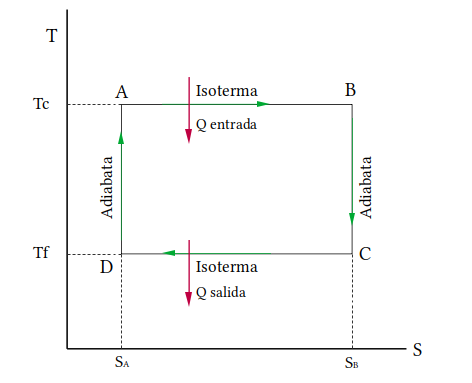
\includegraphics[width=0.60\textwidth]{T-S.png}
                        \caption{Diagrama de un ciclo de Carnot para un gas ideal 
                        en el plano \ut{T - S}}
                        \label{fig:ccst}
                  \end{figure}
            }

      \item  Como se trata de un proceso reversible  sabemos que:
            \[ \dbar Q =TdS \]
            El proceso de $A$ a $B$ se trata de un proceso isotermico, por lo que si integramos la expresión anterior tenemos:
            \[ \int \dbar Q =T_{c}\int dS \]
            \[ \Rightarrow \int _{v_A} ^{v_B} \dbar Q = T_{c} \Delta S\]
            \[nRT_c \ln \left( \frac{v_B}{v_A}\right) = T_{c}\Delta S = Q_{entrada}\]
            En el proceso de $B$ a $C$ al tratarse de un proceso adiabático, no hay intercambio de calor $\Rightarrow Q=0$\\

            En  el proceso de $C$ a $D$ tenemos un proceso isotermico, por lo que analogamente al proceso de $A$ a $B$ tenemos:

            \[ \int \dbar Q =T_{f}\int dS \]
            \[ \Rightarrow \int _{v_C} ^{v_D} \dbar Q = T_{f} \Delta S\]
            \[nRT_f \ln \left( \frac{v_D}{v_C}\right) = T_{f}\Delta S = Q_{salida}\]

            Como se trata de un calor de salida
            \[Q_{salida}=-nRT_c \ln \left( \frac{v_D}{v_C}\right)\]


            Ahora bien si  se trata de un gas ideal y el proceso se realiza a presión constante tenemos que:
            \[ \frac{v_1}{T_1}=\frac{v_2}{T_2}\]
            \[\Rightarrow \frac{T_2}{T_1}=\frac{v_2}{v_1}\]

            Entonces tenemos que:
            \[ \frac{v_B}{v_A}=\frac{Tf}{Tc}=\frac{v_D}{v_c}\]

            Tenemos que la eficiencia esta dada por:
            \[ \eta = \frac{Q_{entrada}+ Q_{salida}}{Q_{entrada}}\]

            \[\Rightarrow  \eta = \frac{nRT_c \ln \left( \frac{v_B}{v_A}\right)-nRT_f \ln \left( \frac{v_D}{v_C}\right)}{nRT_c \ln \left( \frac{v_B}{v_A}\right)}\]
            \[\Rightarrow  \eta = \frac{nRT_c \ln \left( \frac{v_B}{v_A}\right)-nRT_f \ln \left( \frac{v_B}{v_A}\right)}{nRT_c \ln \left( \frac{v_B}{v_A}\right)}\]
            \[\eta =\frac{T_c-T_f}{T_c}\]





\end{enumerate}


    \vspace{\baselineskip}

    %==================================================================%
    % Ejercicio 4
    %==================================================================%
    \item{Un recipiente con N moles de gas ideal con un volumen inicial V\textsubscript{i} esta en contacto con un
                depósito de calor T\textsubscript{0} \ut{K}. El gas se expande isotérmicamente a un volumen V\textsubscript{f}. Calcular:

                \begin{enumerate}[label=\textbf{\alph* )}]
                    \item La cantidad de calor absorbido por el gas, en esta expansión.
                    \item El aumento en la Entropía del gas.
                \end{enumerate}
          }

    
Se puede apreciar que el gas al ser expandido isotérmicamente sufrió un proceso reversible, esto debido a que
conocemos el camino por el cual llego a esa diferencia de volúmenes.

\begin{enumerate}[label=\textbf{\alph* )}]
    \item{De la primer ley de la termodinámica, tenemos para una isoterma que:
    
    \begin{gather*}
        \Delta U\ =\ 0\ \ \ \Rightarrow\\
        Q\ =\ -W\ \ \ \therefore\\
        \\
        Q\ =\ \int_{V_{i}}^{V_{f}} p\ dV\ =\ nRT_{i} \int_{V_{i}}^{V_{f}} \frac{1}{V}\ dV\ =\ 
        \boxed{nRT_{i} \ln{\left(\frac{V_{f}}{V_{i}}\right)}}
    \end{gather*}
     } 

    \item{ al ser un proceso reversible tenemos la siguiente relación 
    
    \begin{equation}
        \int \frac{dQ}{T}\ =\ \int dS\ \ \ \Rightarrow\ \ \  \Delta S\ =\ \frac{Q}{T}
    \end{equation}
    
    Como tenemos un proceso isotérmico 

    \begin{equation*}   
        \boxed{\Delta S\ =\ nR\ln{\left(\frac{V_{f}}{V_{i}}\right)}}
    \end{equation*}
    }
\end{enumerate}

    \vspace{\baselineskip}

\end{enumerate}

\printbibliography[title={Referencias.}]

\end{document}
